\documentclass{standalone}
\usepackage{tikz}
\usetikzlibrary{patterns, positioning}

\begin{document}
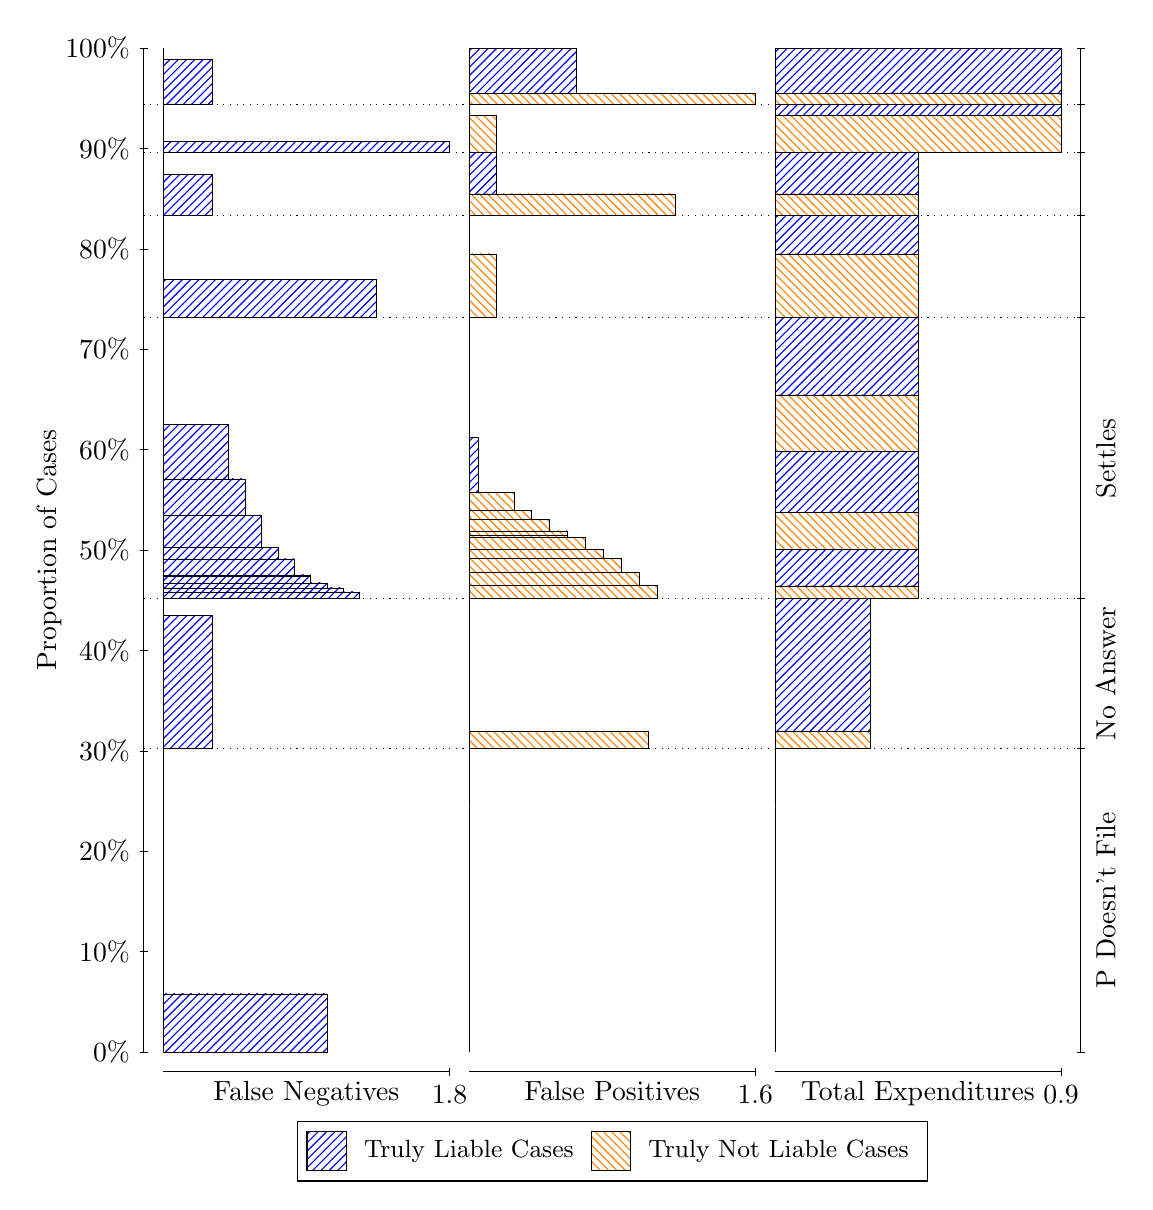
\begin{tikzpicture}
\draw[black, very thin] (1.5,1.75) -- (1.5,14.5);
\node[rotate=90, anchor=center] at (0.3, 8.125) {Proportion of Cases};
\draw[black, very thin] (1.45,1.75) -- (1.55,1.75);
\node[anchor=east] at (1.45, 1.75) {0\%};
\draw[black, very thin] (1.45,3.025) -- (1.55,3.025);
\node[anchor=east] at (1.45, 3.025) {10\%};
\draw[black, very thin] (1.45,4.3) -- (1.55,4.3);
\node[anchor=east] at (1.45, 4.3) {20\%};
\draw[black, very thin] (1.45,5.575) -- (1.55,5.575);
\node[anchor=east] at (1.45, 5.575) {30\%};
\draw[black, very thin] (1.45,6.85) -- (1.55,6.85);
\node[anchor=east] at (1.45, 6.85) {40\%};
\draw[black, very thin] (1.45,8.125) -- (1.55,8.125);
\node[anchor=east] at (1.45, 8.125) {50\%};
\draw[black, very thin] (1.45,9.4) -- (1.55,9.4);
\node[anchor=east] at (1.45, 9.4) {60\%};
\draw[black, very thin] (1.45,10.675) -- (1.55,10.675);
\node[anchor=east] at (1.45, 10.675) {70\%};
\draw[black, very thin] (1.45,11.95) -- (1.55,11.95);
\node[anchor=east] at (1.45, 11.95) {80\%};
\draw[black, very thin] (1.45,13.225) -- (1.55,13.225);
\node[anchor=east] at (1.45, 13.225) {90\%};
\draw[black, very thin] (1.45,14.5) -- (1.55,14.5);
\node[anchor=east] at (1.45, 14.5) {100\%};

\draw[black, very thin] (13.4,1.75) -- (13.4,14.5);
\draw[black, very thin] (13.35,1.75) -- (13.45,1.75);
\node[anchor=west] at (13.35, 1.75) {};
\draw[black, very thin] (13.35,5.6076) -- (13.45,5.6076);
\node[anchor=west] at (13.35, 5.6076) {};
\draw[black, very thin] (13.35,7.5064) -- (13.45,7.5064);
\node[anchor=west] at (13.35, 7.5064) {};
\draw[black, very thin] (13.35,11.077) -- (13.45,11.077);
\node[anchor=west] at (13.35, 11.077) {};
\draw[black, very thin] (13.35,12.372) -- (13.45,12.372);
\node[anchor=west] at (13.35, 12.372) {};
\draw[black, very thin] (13.35,13.177) -- (13.45,13.177);
\node[anchor=west] at (13.35, 13.177) {};
\draw[black, very thin] (13.35,13.784) -- (13.45,13.784);
\node[anchor=west] at (13.35, 13.784) {};
\draw[black, very thin] (13.35,14.5) -- (13.45,14.5);
\node[anchor=west] at (13.35, 14.5) {};

\draw[black, very thin, pattern color=blue, pattern=north east lines] (1.75,1.75) rectangle (3.8262,2.4888);
\draw[black, very thin, pattern color=orange, pattern=north west lines] (1.75,2.4888) rectangle (1.75,5.6076);
\draw[black, very thin, pattern color=blue, pattern=north east lines] (1.75,5.6076) rectangle (2.3729,7.2947);
\draw[black, very thin, pattern color=orange, pattern=north west lines] (1.75,7.2947) rectangle (1.75,7.5064);
\draw[black, very thin, pattern color=blue, pattern=north east lines] (1.75,7.5064) rectangle (4.2414,7.5918);
\draw[black, very thin, pattern color=blue, pattern=north east lines] (1.75,7.5918) rectangle (4.0338,7.644);
\draw[black, very thin, pattern color=blue, pattern=north east lines] (1.75,7.644) rectangle (3.8262,7.7082);
\draw[black, very thin, pattern color=blue, pattern=north east lines] (1.75,7.7082) rectangle (3.6186,7.7921);
\draw[black, very thin, pattern color=blue, pattern=north east lines] (1.75,7.7921) rectangle (3.6186,7.8098);
\draw[black, very thin, pattern color=blue, pattern=north east lines] (1.75,7.8098) rectangle (3.411,8.0108);
\draw[black, very thin, pattern color=blue, pattern=north east lines] (1.75,8.0108) rectangle (3.2033,8.1627);
\draw[black, very thin, pattern color=blue, pattern=north east lines] (1.75,8.1627) rectangle (2.9957,8.5677);
\draw[black, very thin, pattern color=blue, pattern=north east lines] (1.75,8.5677) rectangle (2.7881,9.0291);
\draw[black, very thin, pattern color=blue, pattern=north east lines] (1.75,9.0291) rectangle (2.5805,9.725);
\draw[black, very thin, pattern color=orange, pattern=north west lines] (1.75,9.725) rectangle (1.75,11.077);
\draw[black, very thin, pattern color=blue, pattern=north east lines] (1.75,11.077) rectangle (4.449,11.564);
\draw[black, very thin, pattern color=orange, pattern=north west lines] (1.75,11.564) rectangle (1.75,12.372);
\draw[black, very thin, pattern color=blue, pattern=north east lines] (1.75,12.372) rectangle (2.3729,12.9);
\draw[black, very thin, pattern color=orange, pattern=north west lines] (1.75,12.9) rectangle (1.75,13.177);
\draw[black, very thin, pattern color=blue, pattern=north east lines] (1.75,13.177) rectangle (5.3833,13.318);
\draw[black, very thin, pattern color=orange, pattern=north west lines] (1.75,13.318) rectangle (1.75,13.784);
\draw[black, very thin, pattern color=blue, pattern=north east lines] (1.75,13.784) rectangle (2.3729,14.358);
\draw[black, very thin, pattern color=orange, pattern=north west lines] (1.75,14.358) rectangle (1.75,14.5);
\draw[black, very thin, pattern color=orange, pattern=north west lines] (5.6333,1.75) rectangle (5.6333,4.8688);
\draw[black, very thin, pattern color=blue, pattern=north east lines] (5.6333,4.8688) rectangle (5.6333,5.6076);
\draw[black, very thin, pattern color=orange, pattern=north west lines] (5.6333,5.6076) rectangle (7.9042,5.8194);
\draw[black, very thin, pattern color=blue, pattern=north east lines] (5.6333,5.8194) rectangle (5.6333,7.5064);
\draw[black, very thin, pattern color=orange, pattern=north west lines] (5.6333,7.5064) rectangle (8.0177,7.6757);
\draw[black, very thin, pattern color=orange, pattern=north west lines] (5.6333,7.6757) rectangle (7.7906,7.8374);
\draw[black, very thin, pattern color=orange, pattern=north west lines] (5.6333,7.8374) rectangle (7.5635,8.0164);
\draw[black, very thin, pattern color=orange, pattern=north west lines] (5.6333,8.0164) rectangle (7.3365,8.1312);
\draw[black, very thin, pattern color=orange, pattern=north west lines] (5.6333,8.1312) rectangle (7.1094,8.2838);
\draw[black, very thin, pattern color=orange, pattern=north west lines] (5.6333,8.2838) rectangle (6.8823,8.3067);
\draw[black, very thin, pattern color=orange, pattern=north west lines] (5.6333,8.3067) rectangle (6.8823,8.3681);
\draw[black, very thin, pattern color=orange, pattern=north west lines] (5.6333,8.3681) rectangle (6.6552,8.5132);
\draw[black, very thin, pattern color=orange, pattern=north west lines] (5.6333,8.5132) rectangle (6.4281,8.6246);
\draw[black, very thin, pattern color=orange, pattern=north west lines] (5.6333,8.6246) rectangle (6.201,8.8582);
\draw[black, very thin, pattern color=blue, pattern=north east lines] (5.6333,8.8582) rectangle (5.7469,9.5542);
\draw[black, very thin, pattern color=blue, pattern=north east lines] (5.6333,9.5542) rectangle (5.6333,11.077);
\draw[black, very thin, pattern color=orange, pattern=north west lines] (5.6333,11.077) rectangle (5.974,11.885);
\draw[black, very thin, pattern color=blue, pattern=north east lines] (5.6333,11.885) rectangle (5.6333,12.372);
\draw[black, very thin, pattern color=orange, pattern=north west lines] (5.6333,12.372) rectangle (8.2448,12.649);
\draw[black, very thin, pattern color=blue, pattern=north east lines] (5.6333,12.649) rectangle (5.974,13.177);
\draw[black, very thin, pattern color=orange, pattern=north west lines] (5.6333,13.177) rectangle (5.974,13.643);
\draw[black, very thin, pattern color=blue, pattern=north east lines] (5.6333,13.643) rectangle (5.6333,13.784);
\draw[black, very thin, pattern color=orange, pattern=north west lines] (5.6333,13.784) rectangle (9.2667,13.926);
\draw[black, very thin, pattern color=blue, pattern=north east lines] (5.6333,13.926) rectangle (6.9958,14.5);
\draw[black, very thin, pattern color=orange, pattern=north west lines] (9.5167,1.75) rectangle (9.5167,4.8688);
\draw[black, very thin, pattern color=blue, pattern=north east lines] (9.5167,4.8688) rectangle (9.5167,5.6076);
\draw[black, very thin, pattern color=orange, pattern=north west lines] (9.5167,5.6076) rectangle (10.728,5.8194);
\draw[black, very thin, pattern color=blue, pattern=north east lines] (9.5167,5.8194) rectangle (10.728,7.5064);
\draw[black, very thin, pattern color=orange, pattern=north west lines] (9.5167,7.5064) rectangle (11.333,7.6682);
\draw[black, very thin, pattern color=blue, pattern=north east lines] (9.5167,7.6682) rectangle (11.333,8.1296);
\draw[black, very thin, pattern color=orange, pattern=north west lines] (9.5167,8.1296) rectangle (11.333,8.5988);
\draw[black, very thin, pattern color=blue, pattern=north east lines] (9.5167,8.5988) rectangle (11.333,9.3745);
\draw[black, very thin, pattern color=orange, pattern=north west lines] (9.5167,9.3745) rectangle (11.333,10.095);
\draw[black, very thin, pattern color=blue, pattern=north east lines] (9.5167,10.095) rectangle (11.333,11.077);
\draw[black, very thin, pattern color=orange, pattern=north west lines] (9.5167,11.077) rectangle (11.333,11.885);
\draw[black, very thin, pattern color=blue, pattern=north east lines] (9.5167,11.885) rectangle (11.333,12.372);
\draw[black, very thin, pattern color=orange, pattern=north west lines] (9.5167,12.372) rectangle (11.333,12.649);
\draw[black, very thin, pattern color=blue, pattern=north east lines] (9.5167,12.649) rectangle (11.333,13.177);
\draw[black, very thin, pattern color=orange, pattern=north west lines] (9.5167,13.177) rectangle (13.15,13.643);
\draw[black, very thin, pattern color=blue, pattern=north east lines] (9.5167,13.643) rectangle (13.15,13.784);
\draw[black, very thin, pattern color=orange, pattern=north west lines] (9.5167,13.784) rectangle (13.15,13.926);
\draw[black, very thin, pattern color=blue, pattern=north east lines] (9.5167,13.926) rectangle (13.15,14.5);
\draw[black, dotted] (1.5,5.6076) -- (13.4,5.6076);
\draw[black, dotted] (1.5,7.5064) -- (13.4,7.5064);
\draw[black, dotted] (1.5,11.077) -- (13.4,11.077);
\draw[black, dotted] (1.5,12.372) -- (13.4,12.372);
\draw[black, dotted] (1.5,13.177) -- (13.4,13.177);
\draw[black, dotted] (1.5,13.784) -- (13.4,13.784);
\draw[black, very thin] (1.75,1.5) -- (5.3833,1.5);
\node[anchor=north] at (3.5667, 1.5) {False Negatives};
\draw[black, very thin] (5.3833,1.45) -- (5.3833,1.55);
\node[anchor=north] at (5.3833, 1.45) {1.8};

\draw[black, very thin] (5.6333,1.5) -- (9.2667,1.5);
\node[anchor=north] at (7.45, 1.5) {False Positives};
\draw[black, very thin] (9.2667,1.45) -- (9.2667,1.55);
\node[anchor=north] at (9.2667, 1.45) {1.6};

\draw[black, very thin] (9.5167,1.5) -- (13.15,1.5);
\node[anchor=north] at (11.333, 1.5) {Total Expenditures};
\draw[black, very thin] (13.15,1.45) -- (13.15,1.55);
\node[anchor=north] at (13.15, 1.45) {0.9};

\node[black, centered, rotate=90] at (13.72, 3.6788) {P Doesn't File};
\node[black, centered, rotate=90] at (13.72, 6.557) {No Answer};
\node[black, centered, rotate=90] at (13.72, 9.2916) {Settles};





\draw (7.449999999999999,1.5) node[draw=none] (baseCoordinate) {};
\begin{scope}[align=center]
        \matrix[scale=0.5, draw=black, below=0.5cm of baseCoordinate, nodes={draw}, column sep=0.1cm]{
            \node[rectangle, draw, minimum width=0.5cm, minimum height=0.5cm, pattern=north east lines, pattern color=blue] {}; &
            \node[draw=none, font=\small] (B) {Truly Liable Cases}; &
            \node[rectangle, draw, minimum width=0.5cm, minimum height=0.5cm, pattern=north west lines, pattern color=orange] {}; &
            \node[draw=none, font=\small] (B) {Truly Not Liable Cases}; \\
            };
\end{scope}

\end{tikzpicture}
\end{document}